\subsubsection{Modelo: Servicios de comunicación base}

El modelo servicios de comunicación, representa las bases del protocolo de comunicación entre dispositivos \gls{iot} y una serie de servidores centrales o distribuidos.

Como puede observarse en la figura \ref{fig:modelo_servicios_comunicacion_classes}, tenemos la clase principal \textit{Packet}, que contiene los elementos base del protocolo de comunicación: número de secuencia, \gls{timestamp}, servicios.

Un paquete contiene dentro de su \gls{payload} uno o varios servicios, definidos posteriormente en los posteriores modelos.

Este diseño se ha realizado de esta forma ya que puede ser habitual que un dispositivo no tenga conexión con el servidor de forma continua, teniendo este que guardar toda la comunicación en su memoria a largo plazo para posteriormente cuando consigue conexión, reenviar toda esta información.
Al poder utilizar un solo paquete, simplificamos la comunicación al poder reenviar toda esta comunicación en un solo paso.
Igualmente reducimos la sobrecarga en el protocolo subyacente \gls{tcp}, acumulando varios servicios de información en un solo paquete.

También hemos definido los conceptos petición \textit{ServiceRequest}, respuesta a una petición \textit{ServiceResponse} y notificación sin respuesta previa \textit{ServiceNotification} que se utilizarán en otros modelos de comunicación.

A continuación mostramos en la figura \ref{fig:modelo_servicios_comunicacion_classes}, como se visualiza este modelo en otro tipo de visualización en este caso una vista del diagrama de clases generado, con sus tipos de datos y junto a su documentación, todo ello partiendo siempre del mismo modelo \gls{ecore}. 

\begin{figure}
	\centering
    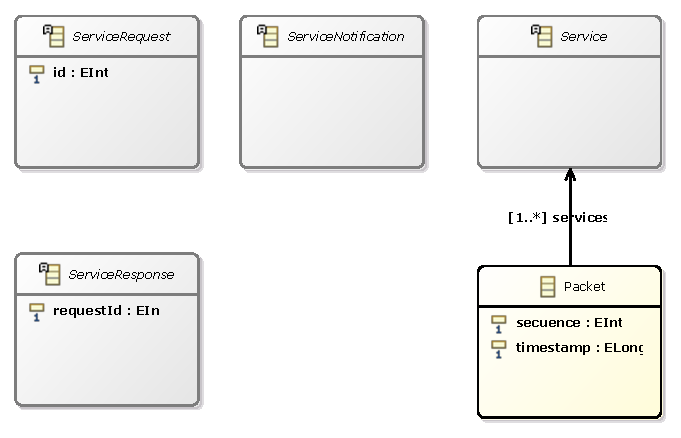
\includegraphics[height=0.3\textheight]{images/models/communications_class_diagram.pdf}
    \captionmodeloclase{Servicios de comunicación}
    \label{fig:modelo_servicios_comunicacion_classes}
\end{figure}
